\newpage
\section{Conclusion}
\label{sec:conclusion}

By analysing the circuit theoretically and then simulating the circuit using Ngspice, we can verify that the values of the unknown components match almost perfectly and all approaches agree on the final currents' directions across the circuit's branches (which can be seen below in figure~\ref{fig:circuit_final}).

\begin{figure}[!ht] \centering
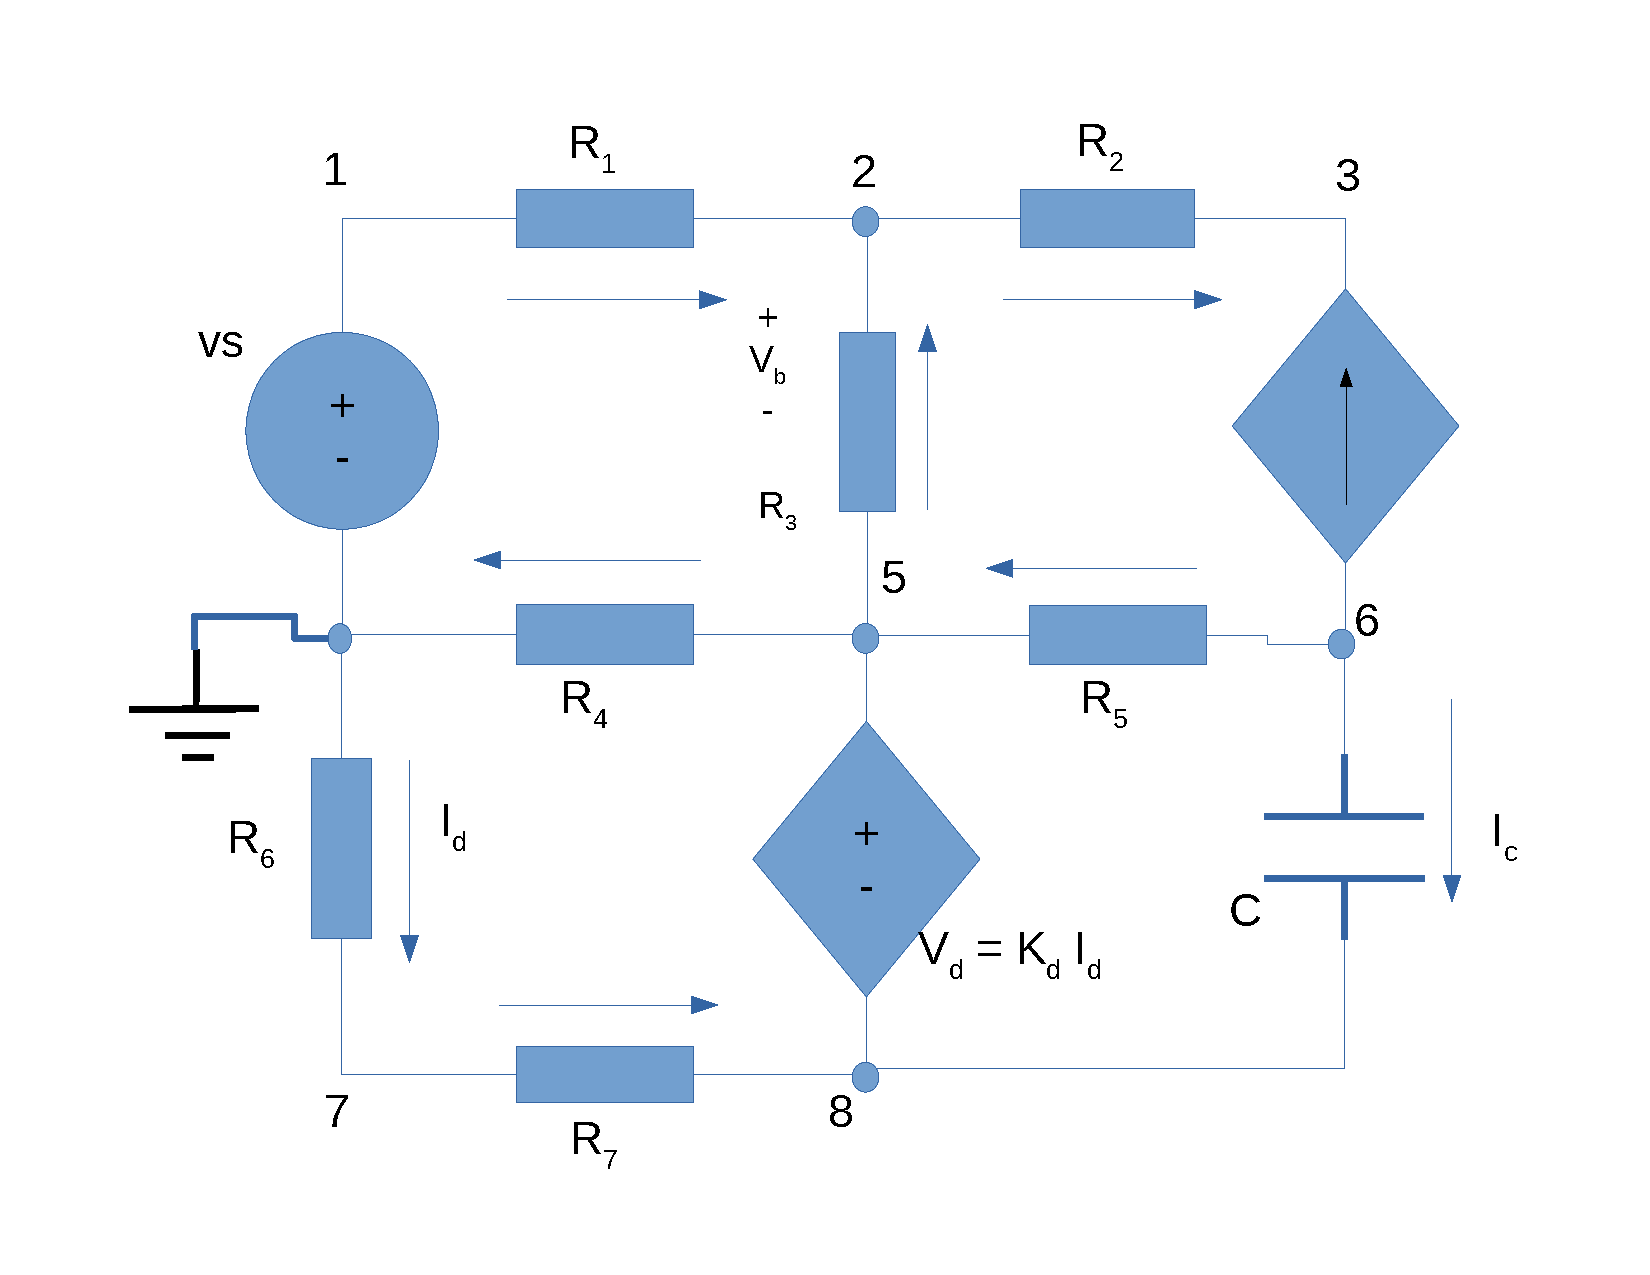
\includegraphics[width=0.8\linewidth]{circuit_final.pdf}
\caption{Representation of the final circuit with all the correct directions for the currents.}
\label{fig:circuit_final}
\end{figure}

To better understand the discrepancies and compare results we present the several tables obtained side by side on octave and ngspice, respectively, in tables \ref{tab:conclusion 1} to \ref{tab:conclusion 2}.





Some small discrepancies are due to the different number of decimal places considered by Octave and Ngspice leading to slight inaccuracies. However, considering that the circuit complexity is still not considered, the differences are negligible. Furthermore, any differences in the order of $10^{-15}$ (or lower), are very likely related to the way the computer programs deal with mathematical operations (seen that $10^{-15}$ is extremely close to the precision of a double's mantissa). Note that the format of the data presented in the Ngspice tables are automatically chosen by the program.

All of this leads to the conclusion that the making of this laboratory assignment was coherent and that the main goal was attained: to achieve the circuit analysis through a theoretical and simulated approach.
